\documentclass{beamer}
\usetheme{CambridgeUS}
\usecolortheme{beaver}
\setbeamertemplate{navigation symbols}{}
\setbeamertemplate{sections/subsections in toc}[circle]
\setbeamertemplate{blocks}[framed]
\beamertemplatetransparentcoveredmedium
\setbeamertemplate{itemize items}[default]
\definecolor{mygrey}{HTML}{D9D9D9}
\setbeamercolor{block title alerted}{use=structure,fg=white,bg=mygrey}

% \includeonlyframes{title,light_harvesting}

\usepackage[utf8x]{inputenc}
\usepackage[english]{babel}
\usepackage{graphicx}
\usepackage{url}
\usepackage{multimedia}
\usepackage{amsmath, calc}
\DeclareGraphicsExtensions{.png}

\usepackage{ifthen}

\usepackage{tikz}
\usetikzlibrary{decorations,arrows}
\usetikzlibrary{decorations.pathmorphing}
\usepgflibrary{decorations.pathreplacing}
\usetikzlibrary{decorations.fractals}
\tikzstyle{every picture}+=[remember picture]
\everymath{\displaystyle}
\tikzstyle{na} = [baseline=-.5ex]

\usepackage[backend=bibtex, style=authoryear-comp]{biblatex}
\addbibresource{references.bib}

\usepackage{xcolor}
\newcommand{\cone}{\color{red}}
\newcommand{\ctwo}{\color{blue}}
\newcommand{\cthree}{\color{purple}}
\newcommand{\customcite}[1]{\citeauthor{#1}, \citetitle{#1}, \citeyear{#1}}
%%%%%%%%%%%%%%%%%%%%%%%%%%%%%%%%%%%%%%%%%%%%%%%%%%%%%%%%%%%%%%%%%%%%%%%%%%%%%%%%
\makeatother

\setbeamertemplate{footline} {%
  \leavevmode%
}

\makeatletter


\newcommand\blfootnote[1]{%
  \begingroup
  \renewcommand\thefootnote{}\footnote{\hspace{-.6cm}\tiny#1}%
  \addtocounter{footnote}{-1}%
  \endgroup
}


\newcommand{\headerwithoutnumbering}{%
  \makeatother
  \setbeamertemplate{headline} {%
    \leavevmode%
    \hbox{%
      \begin{beamercolorbox}[wd=.4\paperwidth,ht=2.25ex,dp=1ex,right]{section in head/foot}%
        \usebeamerfont{section in head/foot}\insertsection\hspace*{1em}
      \end{beamercolorbox}%
      \begin{beamercolorbox}[wd=.6\paperwidth,ht=2.25ex,dp=1ex,left]{subsection in head/foot}%
        \hspace*{1em}\usebeamerfont{subsection in head/foot}\insertsubsection
      \end{beamercolorbox}%
    }
  }
}
\newcommand{\headerwithnumbering}{%
  \makeatother
  \setbeamertemplate{headline} {%
    \leavevmode%
    \hbox{%
      \begin{beamercolorbox}[wd=.4\paperwidth,ht=2.25ex,dp=1ex,right]{section in head/foot}%
        \usebeamerfont{section in head/foot}\insertsection\hspace*{1em}
      \end{beamercolorbox}%
      \begin{beamercolorbox}[wd=.45\paperwidth,ht=2.25ex,dp=1ex,left]{subsection in head/foot}%
        \hspace*{1em}\usebeamerfont{subsection in head/foot}\insertsubsection
      \end{beamercolorbox}%
      \begin{beamercolorbox}[wd=.15\paperwidth,ht=2.25ex,dp=1ex,right]{subsection in head/foot}%
        \insertframenumber{} / \inserttotalframenumber\hspace*{1em}
      \end{beamercolorbox}%
    }
  }
}

\newsavebox{\longestsec}% Box to save longest sectional heading
%%%%%%%%%%%%%%%%%%%%%%%%%%%%%%%%%%%%%%%%%%%%%%%%%%%%%%%%%%%%%%%%%%%%%%%%%%%%%%%%
\title{Hierarchy of Pure States applied to\\Photosynthetic Complexes}
\author{Daniel Süß}
\date{November 22nd, 2013}

\newcommand{\ket}[1]{| #1 \rangle}
\newcommand{\bra}[1]{\langle #1 |}
\newcommand{\Hel}{H_\mathrm{el}}
\newcommand{\opH}[1]{H_\mathrm{#1}}
\newcommand{\opHH}[1]{\mathcal{H}_\mathrm{#1}}
\newcommand{\ptr}{\mathrm{Tr}_\mathrm{env}}
\newcommand{\ii}{\mathrm{i}}
\newcommand{\adj}[1]{#1^{\dagger}}
\newcommand{\cc}[1]{{#1}^\ast}
\newcommand{\quotes}[1]{``#1''}
\newcommand{\dd}{\mathrm{d}}
\renewcommand{\vec}[1]{\mathbf{#1}}
\newcommand{\abs}[1]{\vert #1 \vert}


\newcommand{\zz}{{\vec z}}               % Our noise process
\newcommand{\ZZ}{\cc{Z}}               % Our noise process
\newcommand{\tildeZZ}{\cc{\tilde Z}}
\newcommand{\adjZZ}{\mathcal{D}}         % and it's adjoint

\newcommand{\E}[1][\empty]{%
  \ifthenelse{\equal{#1}{\empty}}
  {\mathbb{E}}
  {\mathbb{E}\left( #1 \right)}
}
\newcommand{\unit}{\mathrm{I}}

\renewcommand{\exp}[1][\empty]{%
  \ifthenelse{\equal{#1}{\empty}}
    {\mathrm{exp}}
    {\mathrm{e}^{#1}}
}

\newcommand{\braket}[2]{\langle #1 | #2 \rangle}


\newcommand{\psit}[1][\empty]{%
  \ifthenelse{\equal{#1}{\empty}}
    {\psi_t}
    {\psi_t^{(#1)}}
}
\newcommand{\psitz}[1][\empty]{%
  \ifthenelse{\equal{#1}{\empty}}
    {\psi_t(\cc\zz)}
    {\psi_t^{(#1)(\cc\zz)}}
}
\newcommand{\psitZ}[1][\empty]{%
  \ifthenelse{\equal{#1}{\empty}}
    {\psi_t(\ZZ)}
    {\psi_t^{(#1)}(\ZZ)}
}

\newcommand{\NMSSE}{\textsc{NMSSE}}

\begin{document}
% TODO Capitalization headers
% TODO CHeck all section/subsection/frame names!!!
% TODO Fix TOC

\headerwithoutnumbering
\begin{frame}[noframenumbering]
  \titlepage
\end{frame}

\begin{frame}[noframenumbering]{Table of Contents}
  \begin{lrbox}{\longestsec}Last section in the presentation\end{lrbox}% Capture longest title
  \begin{columns}
    \column{.0\textwidth}
    \column{.9\textwidth}
    \begin{minipage}[t]{.9\textwidth}
      \tableofcontents
    \end{minipage}
  \end{columns}
\end{frame}

%%%%%%%%%%%%%%%%%%%%%%%%%%%%%%%%%%%%%%%%%%%%%%%%%%%%%%%%%%%%%%%%%%%%%%%%%%%%%%%%
%%%%%%%%%%%%%%%%%%%%%%%%%%%%%%%%%%%%%%%%%%%%%%%%%%%%%%%%%%%%%%%%%%%%%%%%%%%%%%%%
\section{Introduction}
\label{sec:introduction}
%%%%%%%%%%%%%%%%%%%%%%%%%%%%%%%%%%%%%%%%%%%%%%%%%%%%%%%%%%%%%%%%%%%%%%%%%%%%%%%%
\subsection[Light-Harvesting Complexes]{Light-Harvesting Complexes in Bacteria}
\label{sub:light_harvesting_systems}

\headerwithnumbering
\begin{frame}[label=light_harvesting]{Light-Harvesting Complexes}
  % In light-harvessting bacteria
  % interesting: transport light excitation absorbed at antenna to reaction center
  % Needs to be quick and efficient, otherwise excitation lost
  % picture
  \begin{columns}
    \column[c]{.5\textwidth}
    \begin{figure}
      \includegraphics[width=160pt]{green_bacteria_sketch.png}
    \end{figure}
    \column[c]{.45\textwidth}
    \begin{itemize}
      \item light absorbed at chlorosome antennas; transport to reaction center
      \item thermal noise in biological environment
      \item lifetime $\sim 2-5\,\mathrm{ps}$
    \end{itemize}

  \end{columns}
  \blfootnote{%
    \footsize \url{http://www.pks.mpg.de/~eisfeld/wwww/images/green_bacteria_sketch.png}
  }
\end{frame}

\begin{frame}[label=FMO]{The Fenna-Matthews-Olson Complex}
  % first to be studied and simplest pigment-protein Complex
  % also: remarkably long coherence time --> quantum effects important
  % ==> suitable test object for methods and to gain general knowledge
  % PICTURE (FULL PROTEIN ENVIRONMENT)
  % PICTURE (Only FMO)
  % basic structure; 3 Monomers, each consists of 8 Bacteriochlorophyll (BChls)
  %
  % PICTURE (ZOOM ONLY ONE Monomer)
  % PICTURE (ONLY 7 Bacteriochlorophyll)
  %
  % Role of each BCHLs
  \begin{columns}
    \column[c]{.45\textwidth}
    \centering
    \vspace{-1cm}
    \begin{figure}
      \centering
      \includegraphics<1-1>[width=120pt]{fmo_full}
      \includegraphics<2->[width=120pt]{fmo_trimer}
    \end{figure}

    \column[c]{.55\textwidth}
    \begin{itemize}
      \item found in green sulfur bacteria
      \item simplest pigment-protein complex
      \begin{itemize}
        \item ideal test object
      \end{itemize}
      \item quantum effects
      \uncover<2->{%
      \item 3 identical, weakly coupled monomers + protein environment
      }
    \end{itemize}
  \end{columns}
  \vspace{-.5cm}
  \begin{columns}
    \column[c]{.45\textwidth}
    \centering
    \begin{figure}
      \centering
      \visible<3->{%
        \movie[poster,showcontrols=false]{\includegraphics[width=110pt, height=76pt]{monomer}}{monomer.mp4}
      }
    \end{figure}

    \column[c]{.55\textwidth}
    \begin{itemize}
      \uncover<3->{%
      \item 8 Bacteriochlorophylls (BChls)
        \begin{itemize}
          \item here: neglect BChl 8
        \end{itemize}
      \item Energy received at BChls 1+6 transfered to sink at BChl 3
      }
    \end{itemize}
  \end{columns}
  \uncover<3->{%
  \blfootnote{%
    \customcite{TrCaBl09_fmo_structure} \\
    Image created using \customcite{pymol}
  }
}
\end{frame}

\begin{frame}[label=ElHamiltonian]{Physical Model -- Electronic System}
  % Exciton, only one --> Holstein model
  % electronic Hamiltonian (valid only for zero overlap of electronic wave functions)
  %
  % MOVIE (purely electronic transfer)
  % ==> environment necessary; here: harmonic! (why? It works --> ref and we can do it)
  \begin{columns}
    \column[t]{.55\textwidth}
    \begin{itemize}
      \item separation of electronic and vibrational degrees of freedom
        \begin{itemize}
          \item electronic: valence electrons
          \item vibrational: other electrons, nuclear \textsc{dof}, environment
        \end{itemize}
      \item one excited electronic state $\ket{\pi_n}$ per BChl \emph{(exciton)}
        \[ \Hel = \sum_n \epsilon_n \ket{\pi_n}\bra{\pi_n} + \sum_{m,n} V_{mn} \ket{\pi_m}\bra{\pi_n} \]
      (site energy $\epsilon_n$; int.\ strength $V_{mn}$)
      \uncover<2->{%
      \item no effective transport $\Rightarrow$ influence of environment important
      }
    \end{itemize}

    \column[t]{.05\textwidth}
    \column[t]{.4\textwidth}
    \centering
    \visible<2->{%
      \begin{figure}
        \centering
        \includegraphics[width=130pt]{fmo_free.pdf}
      \end{figure}
      \vspace{-.5cm}
      \begin{figure}
        \centering
        \movie[poster,showcontrols=false]{\includegraphics[width=70pt, height=91pt]{fmo_cryo}}{fmo_free2.mp4}
        % \includegraphics[width=70pt]{fmo_free}
      \end{figure}
    }
  \end{columns}
\end{frame}

%%%%%%%%%%%%%%%%%%%%%%%%%%%%%%%%%%%%%%%%%%%%%%%%%%%%%%%%%%%%%%%%%%%%%%%%%%%%%%%%
\subsection{Markovian Open Quantum Systems}
\label{sub:open_quantum_systems}

\begin{frame}[label=oqs_general]{Open Quantum Systems}
  % PICTURE (OPEN QUANTUM SYSTEM)
  % full Hamiltonian Htot + full initial state Psi_0 --> time evolution unitary (1)
  % way to large, not interested in environment --> relevant quantity: Reduced density operator
  % time evolution given by (1), but for practical intentions, important to obtain closed time evolution for rho
  \centering
  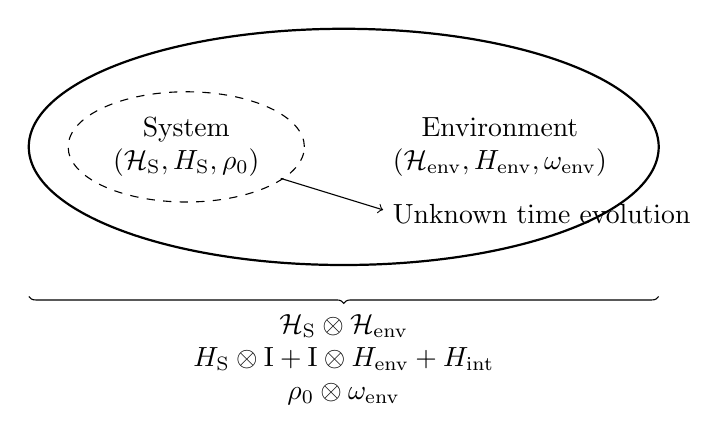
\begin{tikzpicture}
    \visible<1->{%
      \draw[dashed] (0,-0.5) ellipse (1.5 and 0.7);
      \node[align=center] at (0,-0.5) {System\\$(\opHH{S}, \opH{S}, \rho_0)$};
    }

    \visible<1>{%
      \draw [->] (1.2, -0.9) -- (2.5, -1.3) node [right] at (2.5, -1.35) {Unknown time evolution};
    }

    \visible<2->{%
      \draw[thick] (2,-0.5) ellipse (4 and 1.5);
      \node[align=center] [right] at (2.5,-0.5) {Environment\\$(\opHH{env}, \opH{env} , \omega_\mathrm{env})$};
    }

    \visible<3->{%
      \def\y{2}
      \draw[decorate,decoration={brace, mirror}] (-2,-\y.4) -- (6,-\y.4) %
      node[align=center] at (2,-\y.5) [below]{$\opHH{S} \otimes \opHH{env}$ \\ $\opH{S} \otimes \unit + \unit \otimes \opH{env} + \opH{int}$ \\ $\rho_0 \otimes \omega_\mathrm{env}$};
    }
  \end{tikzpicture}
  \visible<4->{%
    \[
      \implies \rho_t = \Lambda_t \rho_0 = \ptr \left(U_t \rho \otimes \omega_\mathrm{env} \adj{U}_t\right)
    \]

    \begin{center}
      $\rightarrow$ Common approach: Derive evolution equation for $\rho_t$.
    \end{center}
  }
\end{frame}

\begin{frame}[label=markov]{Markovian Open Quantum Systems}
  % Assumption: Memoryless, Weak coupling (Born-Markov) --> quantum dynamical semigroup
  % What does this mean?
  % außerdem noch vollständig positiv --> Linblad-Sudarshan-... Master equation
  % Interpretation: Free time evolution + dissipative channels; but not unique
  %
  % PICTURE(FOKKER PLANCK in phase space)
  % --> PICTURE(Langevin in phase space)
  % equivalent stochastic differential equation (only linear form) --> unravelling (not unique)
  % rho recovered as average over pure-state projectors; quantum trajectories
  % short explanation how this is used numerically (Monte Carlo)
  % advantage for numerics: better scaling with system size, easy parallelization (which some people might have noticed on their pc ;)), resulting rho is always a positive operator --> always a genuine state after normalization
  % BUT: Markov approximation too strong: in FMO strong coupling to environment and also eventually long memory times
  \begin{center}
    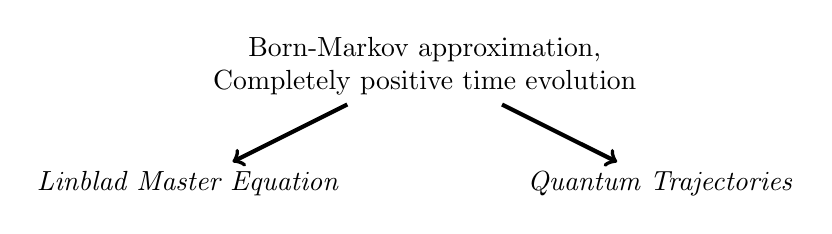
\begin{tikzpicture}
      \node[align=center] at (0, 0) (A) {Born-Markov approximation, \\Completely positive time evolution};
      \node[align=center] at (-3, -1.5) (ME) {\emph{Linblad Master Equation}};
      \draw[->, line width=1.5] (A) -- (ME);
      \node[align=center] at (3, -1.5) (QT) {\emph{Quantum Trajectories}};
      \draw[->, line width=1.5] (A) -- (QT);
    \end{tikzpicture}
  \end{center}
  \uncover<2->{%
    \begin{block}{Linblad Master Equation}
      \[
        \partial_t\rho_t  = - \ii [H, \rho_t] + \Big( [L\,\rho_t, \adj{L}] + [L, \rho_t\,\adj{L}] \Big)
      \]
    \end{block}
    \begin{itemize}
      \item \quotes{free}, unitary time evolution
        + irreversible channel
      \item system of $N^2$ real valued ODEs
    \end{itemize}
  }
\end{frame}


\begin{frame}[label=markov2]{Markovian Open Quantum Systems}
  \begin{block}{Quantum Trajectories (diffusive, linear)}
    \[
      \dd\ket{\psi_t} = \left(-\ii H - \frac{1}{2} \adj{L}L\right) \ket{\psi_t} \dd t + L \ket{\psi_t} \, \dd\cc\xi_t
    \]
  \end{block}
  \begin{itemize}
    \item driven by complex white noise $\dot\xi_t$
    \item $\rho_t$ recovered by \quotes{classical} average over independent realizations
    \[
      \rho_t = \E[\ket{\psi_t}{\bra{\psi_t}}]
      \approx \frac{1}{N} \, \sum_{n=1}^N \ket{\psi^n_t}{\bra{\psi^n_t}}
    \]
    \item system of $2N$ real valued SDEs, trivial parallelization
  \end{itemize}

  \pause
  \begin{center}
    $\rightarrow$ failure of Markovian theory due to strong coupling, \quotes{memory} in time evolution (or initial entanglement)
  \end{center}
\end{frame}

%%%%%%%%%%%%%%%%%%%%%%%%%%%%%%%%%%%%%%%%%%%%%%%%%%%%%%%%%%%%%%%%%%%%%%%%%%%%%%%%
%%%%%%%%%%%%%%%%%%%%%%%%%%%%%%%%%%%%%%%%%%%%%%%%%%%%%%%%%%%%%%%%%%%%%%%%%%%%%%%%
\section{Non-Markovian Open Quantum Systems}
\label{sec:non_markovian_systems}

\headerwithoutnumbering
\begin{frame}[noframenumbering]{Table of Contents}
  \begin{lrbox}{\longestsec}Last section in the presentation\end{lrbox}% Capture longest title
  \begin{columns}
    \column{.0\textwidth}
    \column{.9\textwidth}
    \begin{minipage}[t]{.9\textwidth}
      \tableofcontents[currentsection]
    \end{minipage}
  \end{columns}
\end{frame}

%%%%%%%%%%%%%%%%%%%%%%%%%%%%%%%%%%%%%%%%%%%%%%%%%%%%%%%%%%%%%%%%%%%%%%%%%%%%%%%%
\subsection{Non-Markovian Stochastic Schrödinger Equation}
\label{sub:general_approach}

\headerwithnumbering
\begin{frame}[label=model]{Standard Open System Model}
  % also no general definition of non-Markovianity; for now: evolution equation for reduced density operator not of Linblad form (if it exists)
  % possible reason: strong coupling or "memory" in environment; but also initial entanglement (microscopical derivation of Linblad needs this, not mentioned, because we postulated time evolution)
  % general approach: model environment; derive reduced time evolution by tracing out; no way around microscopical approach
  %
  % Problem to solve (here product initial conditions; zero temperature)
  % EQUATION(Schrödinger)
  % rho_t = Tr_B ...; is there a equation of motion for rho
  %
  % General evolution equation for denisty operator: Najima-Zwanzing
  % EQUATION
  % Problem: Kernel not known in general; even then memory integral impossible not solve numerically
  % Solveable for weak coupling, but general solution not known
  % nonrealtivistic bath of harmonic oscillator, linearly coupled; here: finite number
  % EQUATION
  % Where applicable, Examples#
  % \begin{block}{Nakajima-Zwanzig equation}
  %   \[
  %     \partial_t \rho_t = -\ii \mathcal{L}\rho_t + \int_0^t \mathcal{K}(t-s) \, \rho_{s} \,\dd s
  %   \]
  % \end{block}
  % \vspace{.5cm}
  % transform into interaction picture and use coherent-state representation for psi_t(z) = <z|Psi_t>
  % then equation for Psi_t is equivalent to NMSSE
  % EQUATION(NMSSE)
  % Interpretation: Schrödinger equation for system-bath or for fixed z_\lamdba
  % --> stochastic DGL with driving process Z_t; statistics
  %
  % average taken AFTER propagation
  % EQUATION
  % evaluation by Monte Carlo simulation
  \begin{itemize}
    \item specific model for environment: harmonic oscillators, linearly coupled
      \[
        \opH{tot} = {\cone \opH{sys}}
        + \sum_\lambda {\ctwo \omega_\lambda \adj{a}_\lambda a_\lambda }
        + \sum_\lambda \left( {\cthree \cc{g}_\lambda L \adj{a}_\lambda + g_\lambda \adj{L} a_\lambda } \right)
      \]
    \vspace{-.2cm}
    \pause
    \item interaction picture with respect to $\ctwo \opH{env}$
      \[
        \opH{tot}(t) = {\cone \opH{sys}}
        + \sum_\lambda \left( {\cthree \cc{g}_\lambda L \adj{a}_\lambda \, {\ctwo \exp[\ii \omega_\lambda t]} + g_\lambda \adj{L} a_\lambda \, {\ctwo \exp[-\ii \omega_\lambda t]} } \right)
      \]
    \vspace{-.2cm}
    \pause
    \item Schrödinger equation for system and environment
      \[
        \partial_t \ket{\Psi_t} = -\ii \opH{tot}(t) \ket{\Psi_t}, \qquad \ket{\Psi_0} = \ket{\psi_0} \otimes \ket{0}
      \]
    \item coherent state representation for bath \textsc{dof} $\psitz = \braket{\zz}{\Psi_t}$
    \end{itemize}
\end{frame}


\begin{frame}[label=nonmarkov]{Non-Markovian Stochastic Schrödinger Equation}
  % plays two roles in NMSSE: memory kernel for functional derivative and covariance for stochastic process
  % encodes the complete information about the environent
  % EQUATION(alpha=\sum... = integral
  % by choosing appropriate J(w) we can generate large class of bcfs --> large range of validity from extreme of a single oscillator to Markovian limit:
  %   SSE recovered for alpha = delta --> no "memory time"; Obtained by unphyiscal spectral density J(w) = 1 with negative frequencies; needs further substantiation
  % for what follows we assume exponential alpha --> Lorentzian Spectral density, with negative frequencies; but can also be obtained exactly for T > 0
  \begin{alertblock}{}
    \vspace{-.2cm}
    \[
      \partial_t \only<1-2>{\psitz}\only<3>{\psitZ} = -\ii \opH{sys}\,\only<1-2>{\psitz}\only<3>{\psitZ} + L
      \tikz[baseline]{
        \node[fill=blue!20, anchor=base] (ZZ) {$\ZZ_t$};
      }
      \only<1-2>{\psitz}\only<3>{\psitZ} - \adj{L} \int_0^t
      \tikz[baseline]{
        \node[fill=blue!20, anchor=base] (al) {$\alpha(t-s)$};
      }
     \frac{\delta\only<1-2>{\psitz}\only<3>{\psitZ}}{\delta\ZZ_s} \, \dd s
    \]
  \end{alertblock}
  \begin{itemize}
    \item \quotes{stochastic process}
      \only<1-2>{\tikz[baseline=.4ex]\node (ZZl) {$\ZZ_t = -\ii \sum_\lambda \cc g_\lambda \cc z_\lambda \exp[\ii\omega_\lambda t]$};}
      \only<3->{\tikz[baseline=-.4ex]\node (ZZl) {$\ZZ_t$};}
    \item bath correlation function
      \only<1-2>{$\alpha(t) = \sum_\lambda \abs{g_\lambda}^2 \, \exp[-\ii\omega_\lambda t]$}
      \only<3->{$\alpha(t) = \int_0^\infty J(\omega) \exp[-\ii\omega t] \, \dd \omega$}
    \tikz[na]\node [coordinate] (all) {};

      \vspace{.5cm}
      \uncover<2->{%
      \item only dependence on $\cc z_\lambda$ through $\ZZ_t$ $\Rightarrow$ $\psitz \rightarrow \psitZ$
      }

      \uncover<3->{%
      \item stochastic Schrödinger equation for quantum trajectories $\psitZ$ with
        \[
          \E Z_t = 0, \quad \E[Z_t Z_s] = 0, \quad \mbox{and} \quad \E[Z_t \ZZ_s] = \alpha(t - s)
        \]

        \[
          \rho_t = \ptr \ket{\Psi_t}\bra{\Psi_t} = \E[\ket{\psitZ}\bra{\psitZ}]
        \]
      }
\end{itemize}
  \vspace{-.1cm}
  \blfootnote{%
    \customcite{DiGiSt98_nmqsd}
  }
  \begin{tikzpicture}[overlay]
    \path[->, line width=1] (ZZl) edge [bend left] (ZZ);
    \path[->, line width=1] (all) edge [bend right] (al);
  \end{tikzpicture}
\end{frame}


%%%%%%%%%%%%%%%%%%%%%%%%%%%%%%%%%%%%%%%%%%%%%%%%%%%%%%%%%%%%%%%%%%%%%%%%%%%%%%%%
\subsection{Hierarchy of Pure States}
\label{sub:hops}

\begin{frame}[label=HOPS]{Hierarchy of Pure States (HOPS)}
  % recall NMSSE --> fade to psi^(1); contains all "memory terms" of \dot psi_t
  % with psi^(1) = ...; exponential alpha allows to derive a closed equation for dot\psi^(1)
  % EQUATION
  % ...
  % EQUATION(dotpsi^(k))
  % --> infinite hierarchy of "simple" stochastic differential equations, driven by white noise
  \vspace{-.2cm}
  \begin{equation*}
    \partial_t \psit = -\ii \opH{sys} \psit + L \ZZ_t \psit - \adj{L}
    \color{normal text.fg!15!normal text.bg}
    \only<2->{\color{normal text.fg}}
    \underbrace{\usebeamercolor[fg]{text} \int_0^t \alpha(t-s) \frac{\delta \psit}{\delta\ZZ_s} \, \dd s}_{=:\psit[1]}
  \end{equation*}
  \begin{itemize}
      \pause
    \item closed time evolution equation in case $\alpha(t) = g \,\exp[-\gamma \abs{t} - \ii \Omega t]$
  \end{itemize}
  \vspace{-.2cm}
  \pause
  \begin{block}{}
    \vspace{-.3cm}
    \begin{align*}
      \partial \psit[0] & = (-\ii \opH{sys} + L\ZZ_t) \, \psit[0]                         &                       & -
      \tikz[baseline]{%
        \node [anchor=base] (b0) {$\adj{L}\psit[1]$};
      } \\
      \\
      \partial \psit[1] & = (-\ii \opH{sys} - (\gamma + \ii\Omega) + L\ZZ_t) \, \psit[1]  & + g
      \tikz[baseline]{%
        \node [anchor=base] (a1) {$L \psit[0]$};
      }
      & -
      \tikz[baseline]{%
        \node [anchor=base] (b1) {$\adj{L}\psit[2]$};
      } \\
      & \mathrel{\makebox[\widthof{=}]{\vdots}} \\
      \partial \psit[k] & = (-\ii \opH{sys} - k(\gamma + \ii\Omega) + L\ZZ_t) \, \psit[k] & + k g
      \tikz[baseline]{%
        \node [anchor=base] (ak) {$L \psit[k-1]$};
      }
      & -
      \tikz[baseline]{%
        \node [anchor=base] (bk) {$\adj{L}\psit[k+1]$};
      } \\
      & \mathrel{\makebox[\widthof{=}]{\vdots}}
    \end{align*}
  \end{block}
  \begin{tikzpicture}[overlay]
    \draw[->, color=red, line width=1] (b0) -- ++ (0.0, -1);
    \draw[->, color=red, line width=1] (b1) -- ++ (0.0, -1);
    \draw[->, color=red, line width=1] (bk) -- ++ (0.0, -1);
    \draw[->, color=blue, line width=1] (a1) -- ++ (0.0, 1);
    \draw[->, color=blue, line width=1] (ak) -- ++ (0.0, 1);
  \end{tikzpicture}
\end{frame}


\begin{frame}[label=truncation]{Truncation of the Hierarchy}
  % Got rid of functional derivative by absorbing into infinte number auxillary state
  % --> even more intricate
  % EQUATION(formal solution andeutungsweise, mit colors)
  % for k large enough, can always be written as ... psi^(k-1) - ... psi^(k+1)
  % second supressed by 1/k provided psi^(k+1) is not significantly larger
  % --> cross out psi^(k+1); TERMINATOR
  % Interpreation: plug into psi_t(k); for g = \gamma / 2 --> Markovian SSE, but driven by colored noise
  % hierarchy is expansion around "Markovian environment", but adaptable by simply increasing number of k
  \begin{center}
    \begin{tikzpicture}
      \node at (0.0, 0.0) (f1) {%
        $\partial_t \psit[k] =
        {\cthree (-\ii \opH{sys} - k(\gamma + \ii\Omega) + L\ZZ_t) \, \psit[k] }
        + {\ctwo kg \, L\psit[k-1] }
        - {\cone \adj{L}\psit[k+1] }$
      };
      \node at (0.0, -2) (f2){%
        \only<1>{%
        $\psit[k] = \int_0^t
        {\cthree \exp[-k(\gamma + \ii\Omega)(t-s)] \, \ldots }

          \left(
          {\ctwo kg \, L\psi_s^{(k-1)} }
        - {\cone \adj{L}\psi_s^{(k+1)}  }
        \right) \, \dd s$
      }
        \only<2->{%
        $\psit[k] \sim
          {\ctwo kg \, L\psi_t^{(k-1)} }
        - {\cone \adj{L}\psi_t^{(k+1)}  }
        $
      }
      };
    \draw[<->,double, double distance=.10cm, line width=1, implies-implies] (f1) -- (f2);
    \end{tikzpicture}
  \end{center}



  \uncover<3>{
    \begin{itemize}
      \item truncation at finite order $D$ with \emph{terminator} (here: $\Omega = 0$)
        \begin{align*}
          \partial_t \psit[D] = \left(
            {\cthree -\ii\opH{sys} - D\gamma + L\ZZ_t } - {\cone \frac{g}{\gamma} \adj{L}L }
          \right) \psit[D]
          + {\ctwo Dg \, L \psit[D-1] }
        \end{align*}
      \item \quotes{Markovian} approximation for $D^\mathrm{th}$ order
    \end{itemize}
  }
\end{frame}


\begin{frame}[label=hops_remarks]{Further Remarks}
  % used gamma to surpress, we dont have a simple criterion to obtain hierarchy depth --> check by increasing ±1
  % nonlinear version exists to cope with importance sampling
  % multiple exponential modes: rapid growth of number of aux. states required with Depth of hierarchy
  % for general spectral denisty/bcf and temperature: expansion in exponential alphas possible
  \begin{itemize}
    \item no simple criterion to determine $D$ $\rightarrow$ individual checking necessary
    \item rule of thumb: large truncation order $D$ for
      \begin{itemize}
        \item small memory time $\iff$ large $\gamma$
        \item strong coupling $\iff$ large g
      \end{itemize}
    \pause
    \vspace{.1cm}
    \item nonlinear version $\rightarrow$ proper importance sampling
    \vspace{.1cm}
    \pause
  \item exponential \textsc{bcf} requires negative frequencies $\rightarrow$ unphysical
    \begin{center}
      \begin{tikzpicture}
        \node<1-2>[opacity=.15]{\includegraphics[width=200pt]{lorentzians.pdf}};
        \node<3>[opacity=1.]{\includegraphics[width=200pt]{lorentzians.pdf}};
      \end{tikzpicture}
    \end{center}
  \vspace{-.3cm}
  \item proper treatment for $T \neq 0$
  \end{itemize}
\end{frame}


%%%%%%%%%%%%%%%%%%%%%%%%%%%%%%%%%%%%%%%%%%%%%%%%%%%%%%%%%%%%%%%%%%%%%%%%%%%%%%%%
%%%%%%%%%%%%%%%%%%%%%%%%%%%%%%%%%%%%%%%%%%%%%%%%%%%%%%%%%%%%%%%%%%%%%%%%%%%%%%%%
\section{HOPS applied to the FMO-Complex}
\label{sec:application_to_fmo}

\headerwithoutnumbering
\begin{frame}[noframenumbering]{Table of Contents}
  \begin{lrbox}{\longestsec}Last section in the presentation\end{lrbox}% Capture longest title
  \begin{columns}
    \column{.0\textwidth}
    \column{.9\textwidth}
    \begin{minipage}[t]{.9\textwidth}
      \tableofcontents[currentsection]
    \end{minipage}
  \end{columns}
\end{frame}
%%%%%%%%%%%%%%%%%%%%%%%%%%%%%%%%%%%%%%%%%%%%%%%%%%%%%%%%%%%%%%%%%%%%%%%%%%%%%%%%

\headerwithnumbering
\begin{frame}[label=fmo_model]{The FMO-Complex -- Full Model}
  % Exciton Hamiltonian --> fade in harmonic environent
  % coupling operators, independent environents --> wird haarig
  %
  % spectral density: used here and more realisitic (Wendeling)
  % why? --> established results with HEOM, not so good scaling with Depth, keep number of modes small
  % information about structure and spectral denisty: experimental by spectroscopy; transfer is not measureable
  % site energies --> two distinct channels
  \begin{itemize}
    \item environment: independent, identical harmonic baths for each BChl
    \item all thermal effects included in \emph{thermal correlation function}
      \[
        \alpha(t) = \int_0^\infty J(\omega) \, \left( \coth\left(\frac{\omega}{2T}\right) \cos(\omega t) - \ii \sin(\omega t) \right) \dd\omega
      \]
    \pause
    \vspace{-.5cm}
    \item highly structured realistic spectral density
      \begin{itemize}
        \item large number of exponential modes required
        \item simplified spectral density (for $D=2$: 120 vs.\ 15576 auxiliary states)
      \end{itemize}
      \begin{center}
        \begin{tikzpicture}
          \node<1>[opacity=.15]{\includegraphics[width=160]{spectral.pdf}};
          \node<2>[opacity=1.]{\includegraphics[width=160]{spectral.pdf}};
        \end{tikzpicture}
      \end{center}
  \end{itemize}
  \vspace{-1cm}
  \blfootnote{%
    \customcite{We_fmo}
  }
\end{frame}


\begin{frame}[label=cryogenic]{Exciton Transfer at Cryogenic Temperature}
  % picture with both channels, reference result
  % some short discussion; movie showing wavelike transfer
  \vspace{-.3cm}
  \begin{center}
    \begin{figure}[t]
      \centering
      \includegraphics[width=300pt]{fmo_ishfl.pdf}
    \end{figure}
    \begin{columns}
      \column[c]{.3\textwidth}
      \centering
      \movie[poster,showcontrols=false]{\includegraphics[width=70pt, height=94pt]{fmo_cryo}}{fmo_cryo2.mp4}
      \column[c]{.7\textwidth}
      \begin{itemize}
        \pause
        \item directed energy transfer toward BChls 3 + 4
        \item yield of 40\,\% (resp. 75\,\%) on relevant BChls
        \item coherent, wavelike dynamics up to $t \approx 0.7\,\mathrm{ps}$
      \end{itemize}
    \end{columns}
  \end{center}
  \blfootnote{%
    \customcite{IsFl09_fmo}
  }
\end{frame}


\begin{frame}[label=cryogenic2]{Exciton Transfer at Cryogenic Temperature}
  % picture with both channels, reference result
  % some short discussion; movie showing wavelike transfer
  \begin{center}
    \begin{columns}
      \column[c]{.3\textwidth}
      \centering

      \definecolor{blue}{rgb}{0,0.2,0.8}
      \definecolor{purple}{rgb}{1,0,0.6}
      \definecolor{ffqqqq}{rgb}{1,0,0}
      \definecolor{cyan}{rgb}{0,0.8,0.8}
      \definecolor{grey}{rgb}{0.6,0.6,0.6}
      \definecolor{green}{rgb}{0,1,0}
      \begin{tikzpicture}[line cap=round,line join=round,yscale=1.2, xscale=0.5]
        \begin{footnotesize}
          %% Coordinate axis
          \foreach \y in {200, 300, 400, 500, 600}
          \draw[shift={(-.6, 0.01*\y)},color=black] (2pt,0pt) -- (-2pt,0pt) node[left] {$\y$};
          \draw[color=black] (-2.6, 4.00) node[rotate=90] {$\epsilon_m$ [$cm^{-1}$]};
          \draw[->,color=black,>=triangle 45] (-.6,1.90) -- (-.6,6.50);

          %% Energy levels
          \draw [color=red, line width=1pt] (-.3,4.10)    -- node[below] (1b) {\footnotesize 410} node[above] (1a) {\footnotesize\textbf{1}} ++(.7, 0);
          \draw [color=green, line width=1pt] (0,5.30)    -- node[below] (2b) {\footnotesize 530} node[above] (2a) {\footnotesize\textbf{2}} ++(.7, 0);
          \draw [color=blue, line width=1pt] (1.2,2.10)   -- node[below] (3b) {\footnotesize 210} node[above] (3a) {\footnotesize\textbf{3}} ++(.7, 0);
          \draw [color=purple, line width=1pt] (1.9,3.20) -- node[below] (4b) {\footnotesize 320} node[above] (4a) {\footnotesize\textbf{4}} ++(.7, 0);
          \draw [color=cyan, line width=1pt] (1.8,4.80)   -- node[below] (5b) {\footnotesize 480} node[above] (5a) {\footnotesize\textbf{5}} ++(.7, 0);
          \draw [color=orange, line width=1pt] (2.2,6.30) -- node[below] (6b) {\footnotesize 630} node[above] (6a) {\footnotesize\textbf{6}} ++(.7, 0);
          \draw [color=grey, line width=1pt] (3,4.40)     -- node[below] (7b) {\footnotesize 440} node[above] (7a) {\footnotesize\textbf{7}} ++(.7, 0);

          %% Connecting arrows
          \draw[->, line width=.8pt] (1a) -- (2b);
          \draw[->, line width=.8pt] (2b) -- (3a);
          \draw[->, line width=.8pt] (4b) -- (3a);
          \draw[->, line width=.8pt] (5b) -- (4a);
          \draw[->, line width=.8pt] (7b) -- (4a);
          \draw[->, line width=.8pt] (6b) -- (5a);
          \draw[->, line width=.8pt] (6b) -- (7a);
        \end{footnotesize}
      \end{tikzpicture}
      \column[c]{.7\textwidth}
      \begin{figure}[t]
        \centering
        \includegraphics[width=250pt]{fmo_ishfl.pdf}
      \end{figure}
      \begin{itemize}
        \item two distinct transport channels
        \item potential step between BChls 1 \& 2
          \begin{itemize}
            \pause
            \item higher yield with start on BChl 6
            \item correction in full monomer
            \item assumed to serve as barrier preventing depopulation of target
            \item coherent tunneling may assist overcoming
          \end{itemize}
      \end{itemize}
    \end{columns}
  \end{center}
\end{frame}

\begin{frame}[label=physiological]{Exciton Transfer at Physiological Temperature}
  % picture one channel, with HEOM and HOPS
  % still wavelike even at higher temperature
  % very important since: Comparisson of number of aux states here
  % here vorteil aufgegessen von number of samples required, but for larger systems much better
  \vspace{-.2cm}
  \begin{center}
    \begin{figure}[t]
      \centering
      \includegraphics[width=290pt]{fmo_mevsphi.pdf}
    \end{figure}
  \end{center}
  \vspace{-.3cm}
  \begin{itemize}
    \item same qualitative result as for cryogenic temperature
    \item shorter timespan of wavelike dynamics (up to $t \approx 0.3\,\mathrm{ps}$)
    \item yield reduced by 25\,\%
    \vspace{.1cm}
    \pause
    \item \textsc{HEOM} -- hierarchical equations of motion
    \begin{itemize}
      \item based on density matrix formalism
      \item similar hierarchical structure
    \end{itemize}
  \end{itemize}
  \blfootnote{%
    \customcite{Ta06_stochastic};
    \customcite{StSc12_heom}
  }
\end{frame}

%%%%%%%%%%%%%%%%%%%%%%%%%%%%%%%%%%%%%%%%%%%%%%%%%%%%%%%%%%%%%%%%%%%%%%%%%%%%%%%%
%%%%%%%%%%%%%%%%%%%%%%%%%%%%%%%%%%%%%%%%%%%%%%%%%%%%%%%%%%%%%%%%%%%%%%%%%%%%%%%%
\section{Conclusion \& Outlook}
\label{sec:conclusion_and_outlook}

\headerwithoutnumbering
\begin{frame}[noframenumbering]{Table of Contents}
  \begin{lrbox}{\longestsec}Last section in the presentation\end{lrbox}% Capture longest title
  \begin{columns}
    \column{.0\textwidth}
    \column{.9\textwidth}
    \begin{minipage}[t]{.9\textwidth}
      \tableofcontents[currentsection]
    \end{minipage}
  \end{columns}
\end{frame}

%%%%%%%%%%%%%%%%%%%%%%%%%%%%%%%%%%%%%%%%%%%%%%%%%%%%%%%%%%%%%%%%%%%%%%%%%%%%%%%%

\headerwithnumbering
\begin{frame}[label=summary]{Summary}
  % efficient method to calculate the reduced density operator of an open quatum system coupled to bosonic environent
  % got rid of problematic memory terms by introducing auxillary states, only a finite number needed
  %
  % what can you do with it? here: exciton transfer in simplified model of Photosynthetic complexes
  % seen: even at physiological temperature quantum coherent motion is responsible for high efficiency
  % but underlying standard model also applicable to e.g. ...
  \begin{itemize}
    \item Hierarchy of pure states based on \NMSSE
      \begin{itemize}
        \item applicable to system coupled linearly to bosonic environment
        \item numerically exact and valid for a large parameter regime
        \item solves the \quotes{functional derivative problem} without any approximation
        \item systematic check of convergence
        \item higher precision at equal truncation order than \textsc{HEOM}-approach
      \end{itemize}
    \pause
    \vspace{.3cm}
  \item exciton-energy transfer in light-harvesting complexes
    \begin{itemize}
      \item simplest example: \textsc{FMO}-complex in sulfur bacteria
      \item reproduce established results using \textsc{HOPS}
      \item remarkably high efficiency; possible explanation due to quantum effects
    \end{itemize}
    \pause
    \vspace{.3cm}
  \item We did not talk about...
    \begin{itemize}
      \item nonlinear equations
      \item thermal bath correlation function expansion
      \item absorption spectra
      \item \ldots
    \end{itemize}
  \end{itemize}
\end{frame}


\begin{frame}[label=outlook]{And now what?}
  % application to full complex --> 24 sites with 2 modes possible with HOPS, since only first order required for parameters used (no results from HEOM, only ZOFE -- other problems)
  % --> dont expect qualitatively new behavior due to weak coupling as mentioned before (except for the 8th BChl)
  %
  % more interesting: influence of other bcf, more structure
  %   - established ZOFE results: not so reliable since not checkable
  %   - no HEOM results (my knowledge) since assume also 1st and 4th order -- compare number of aux states
  %
  % Markov SSE unravelling, we started from microscopical model; question: is there connection to HEOM, why HOPS works better?
  %
  % all experimental information form spectroscopy; NMSSE very efficient for absorption spectra/no average necessary
  % --> all the goodies from stochastic pure states without the cons!!!
  % is this expandable to other techniques (e.g. very important: 2D spectroscopy)
  \uncover<1>{%
    \begin{columns}
      \column[c]{.45\textwidth}
      \begin{block}{Exciton Transfer}
        \begin{small}
          \begin{itemize}
            \item larger system size
            \item influence of spectral density
          \end{itemize}
        \end{small}
      \end{block}
      \begin{block}{Numerical Implementation}
        \begin{small}
        \end{small}
      \end{block}
      \column[c]{.45\textwidth}
      \begin{block}{Open Questions}
        \begin{small}
          \begin{itemize}
            \item connection to \textsc{HEOM}
            \item non-exponential \textsc{bcf}s
            \item treatment of experimental accessible quantities
          \end{itemize}
        \end{small}
      \end{block}
    \end{columns}
  }
  \vspace{1cm}
  \begin{center}
    \visible<2>{\huge Thank you for your attention!}
  \end{center}
\end{frame}

{
  \setbeamercolor{background canvas}{bg=black}
  \frame[plain]{}
}

\end{document}
